\documentclass[11pt,twocolumn,letterpaper]{article}

\usepackage{cvpr}
\usepackage{times}
\usepackage{epsfig}
\usepackage{graphicx}
\usepackage{amsmath}
\usepackage{amssymb}

% Include other packages here, before hyperref.

% If you comment hyperref and then uncomment it, you should delete
% egpaper.aux before re-running latex.  (Or just hit 'q' on the first latex
% run, let it finish, and you should be clear).
\usepackage[breaklinks=true,bookmarks=false]{hyperref}

\cvprfinalcopy % *** Uncomment this line for the final submission

%\def\cvprPaperID{****} % *** Enter the CVPR Paper ID here
%\def\httilde{\mbox{\tt\raisebox{-.5ex}{\symbol{126}}}}

% Pages are numbered in submission mode, and unnumbered in camera-ready
%\ifcvprfinal\pagestyle{empty}\fi
\setcounter{page}{1}
\begin{document}

%%%%%%%%% TITLE
\title{Measuring Heart Rate from Video}

\author{Isabel Bush\\
\it{ibush@stanford.edu}\\
Stanford Computer Science\\
353 Serra Mall, Stanford, CA 94305
}
\maketitle
%\thispagestyle{empty}

\section*{Introduction}

A person's heart rate can be indicative of their health, fitness, activity level, stress, and much more. Cardiac pulse is typically measured in clinical settings using electrocardiogram (ECG), which requires patients to wear chest straps with adhesive gel patches that can be abrasive and become uncomfortable for the user. Chest straps are also common for fitness heart-rate monitors used by joggers or other athletes. Heart rate may also be monitored using pulse oximetry sensors that may be worn on the fingertip or earlobe. These sensors are not convenient for long-term wear and the pressure can become uncomfortable over time.

In addition to the discomforts of traditional pulse measurement devices, these devices can damage the fragile skin of premature newborns or elderly people. For these populations especially, a non-contact means of detecting pulse could be very beneficial. Non-contact heart rate measurement through a simple webcam or phone camera would also aid telemedicine and allow the average person to track their heart rate without purchasing special equipment. As part of the recent gain in popularity of fitness apps and the quantified self, regular non-obtrusive monitoring through a computer web camera may help detect changes in a person's heart rate over time and indicate changing health or fitness. 

Heart rate can be detected without contact through photo-plethysmograpy (PPG), which measures variations in blood volume by detecting changes in light reflectance or transmission throughout the cardiovascular pulse cycle. PPG is usually performed with dedicated light sources with red or infrared wavelengths, as is the case for pulse oximetry sensors. 

Verkruysse \etal showed that the plethysmographic signal could also be detected in video from a regular color camera~\cite{Nelson:2008aa}. They found that the signal could be detected within the red, green, and blue channels of color video of exposed skin, but that it was strongest in the green channel, which corresponds to the fact that hemoglobin has absorption peaks for green and yellow light wavelengths. They also found that although the signal could be detected in multiple locations on the body, it was strongest on the face, especially on the forehead.

Although the plethysmographic signal may be detected in the raw color channel data, it is mixed in with other sources of color variation such as changes in ambient light or motion. Poh \etal found that the signal could be better extracted by using independent component analysis (ICA) to separate independent source signals from the mixed color signals~\cite{Poh:2010aa}.

Other studies have shown that color changes in the face due to pulse may be magnified by amplifying small changes between video frames~\cite{Wu:2012aa}, and that heart rate can be detected through vertical head motion in addition to color changes~\cite{Balakrishnan:2013aa}. Although these are interesting new developments in this space, they are less practical for daily or medical use as the former is more for visualization than quantification, and the latter requires the subject to remain very still for accurate measurements.

In this project, I will explore an approach for heart rate detection using RGB color changes in video of faces similar to that done by Poh \etal~\cite{Poh:2010aa}. Time permitting, I may try to improve the accuracy of the algorithm, especially for moving subjects.

\section*{Technical Approach}

Detecting heart rate in video consists of three main steps. First, video clips of various faces must be collected. Second, the facial region must be detected and tracked across each frame of the video since the face is the only portion of the frame that will contain heart rate information. Third, the plethysmographic signal must be extracted from the change in pixel colors within the face region over time and analyzed to determine the prominant frequency within the heart rate range.

\subsection*{Data Collection}

I will collect video data of a few subjects with varying skin-tones and in varying lighting conditions. Each video will be approximately one minute in length and will be taken with a Macbook Pro webcam and/or iPhone camera. Multiple videos of each subject will be taken, some with the subject still, some with the subject moving slightly, and some after the subject has exercised to check heart rate detection at a wider range.

During video recording, subjects will be wearing a finger PPG sensor so that the heart rate results from the video can be compared to a ground truth.

\subsection*{Face Detection and Tracking}

Face detection and tracking is performed using Haar cascade classifiers as proposed by Viola and Jones~\cite{Viola:2001aa} and improved by Lienhart \etal~\cite{Leinhart:2002aa}. The classifiers consist of several simpler classifiers applied in stages to a region of interest (ROI). Each simple classifier contains weighted votes of multiple basic classifiers trained on Haar-like features designed to detect edges, lines, and blobs. Specifically, I use the OpenCV Cascade Classifier pre-trained on positive and negative frontal face images~\cite{opencv_library}. To detect the face in video frames, classification windows of varying sizes are slid across each image frame.

To maintain consistency across frames, if no face is detected in a frame, the face from the previous frame is used, and if multiple faces are detected, the face nearest to that in the previous frame is used. The face detector outputs a bounding box for the face. Initially, I am using the center 60\% of the bounding box width and the full height as my ROI, as was done by Poh \etal~\cite{Poh:2010aa}.

Time-permitting, I may try to improve the face detection and tracking and the estimation of the ROI. I could experiment with detecting other features on the face (eyes for example) and using this as the determination for which face to choose if there are multiple faces detected. I could improve the chosen ROI by segmenting out the facial region within the bounding box to avoid including hair or background in my ROI. I could also remove a region containing the eyes to reduce the non-skin pixels within the ROI, or experiment with segmenting out only the forehead region since that was shown to have strongest plethysmographic signal. Finally, I could try to detect large head movements and ignore the faces found in these frames to reduce the error due to motion.

\subsection*{Heart Rate Detection}

Once I have an ROI for each frame, I can begin to extract the heart rate from the color image data. The first step is to average the pixels in the ROI across each color channel to get three signals $x_R(t)$, $x_G(t)$, and $x_B(t)$ corresponding to the average red, green, and blue facial pixels at time $t$. I then normalize these signals across a 30-second sliding window with a 1-second stride (so the heart rate is re-estimated every second).

I then use ICA to extract the independent source signals from the observed mixed color signals. ICA assumes that the number of source signals is no more than the number of observed signals, so I assume there are three source signals $s_1(t)$, $s_2(t)$, and $s_3(t)$ contributing to the observed color changes in the three channels. ICA assumes the observed mixed signals are a linear combination of these source signals. Although this assumption may not be valid as changes in blood volume and the intensity of reflected light in skin tissue over distance may be nonlinear, for the 30-second time window it should be a reasonable approximation. With this linear approximation for signal mixing, we have 
	$$x(t) = As(t)$$ 
	$$s(t) = A^{-1}x(t)$$
where $x(t) = [x_R(t)\ x_G(t)\ x_B(t)]^T$, $s(t) = [s_1(t)\ s_2(t)\ s_3(t)]^T$, and $A$ is a 3x3 matrix of coefficients. Then ICA attempts to find an approximation of $A^{-1}$ that maximizes the non-Gaussianity of each source. I will use FastICA to recover the approximate source signals $s(t)$.

Once I have the source signals, I can use Fourier transform to examine their power spectrum and determine the prominent signal frequencies. I can isolate frequency peaks in the power spectrum within the range 0.75 to 4 Hz, which corresponds to physiological heart rate ranges of 45 to 240 bpm. Following Poh \etal, I only select spikes within 0.2 Hz of the previous measurement as heart-rates generally change less than 12 bpm over a single second~\cite{Poh:2010aa}. The measured heart rate will be the frequency within the acceptable range corresponding to the peak with the highest magnitude.

\section*{Progress}

I have implemented an initial version of all steps listed in the technical approach section. 

\subsection*{Data Collection}
I initially collected one-minute videos of my face using a MacBook Pro FaceTime HD webcam. After some experimentation, I found that the frame rate of the recorded videos differed depending on the lighting conditions and was never higher than about 12 fps. From some initial investigation, it seems that it is not possible to set the desired frame-rate as it is controlled by proprietary Apple software. 

Since knowing the precise frame rate is crucial to extracting an accurate heart rate, I switched to recording video with an iPhone camera. I collected a couple videos of my face straight-on and in natural lighting at 30 fps. For these initial videos, I tried to remain as still as possible during the recording.

\subsection*{Face Detection and Tracking}

\begin{figure}
\begin{center}
	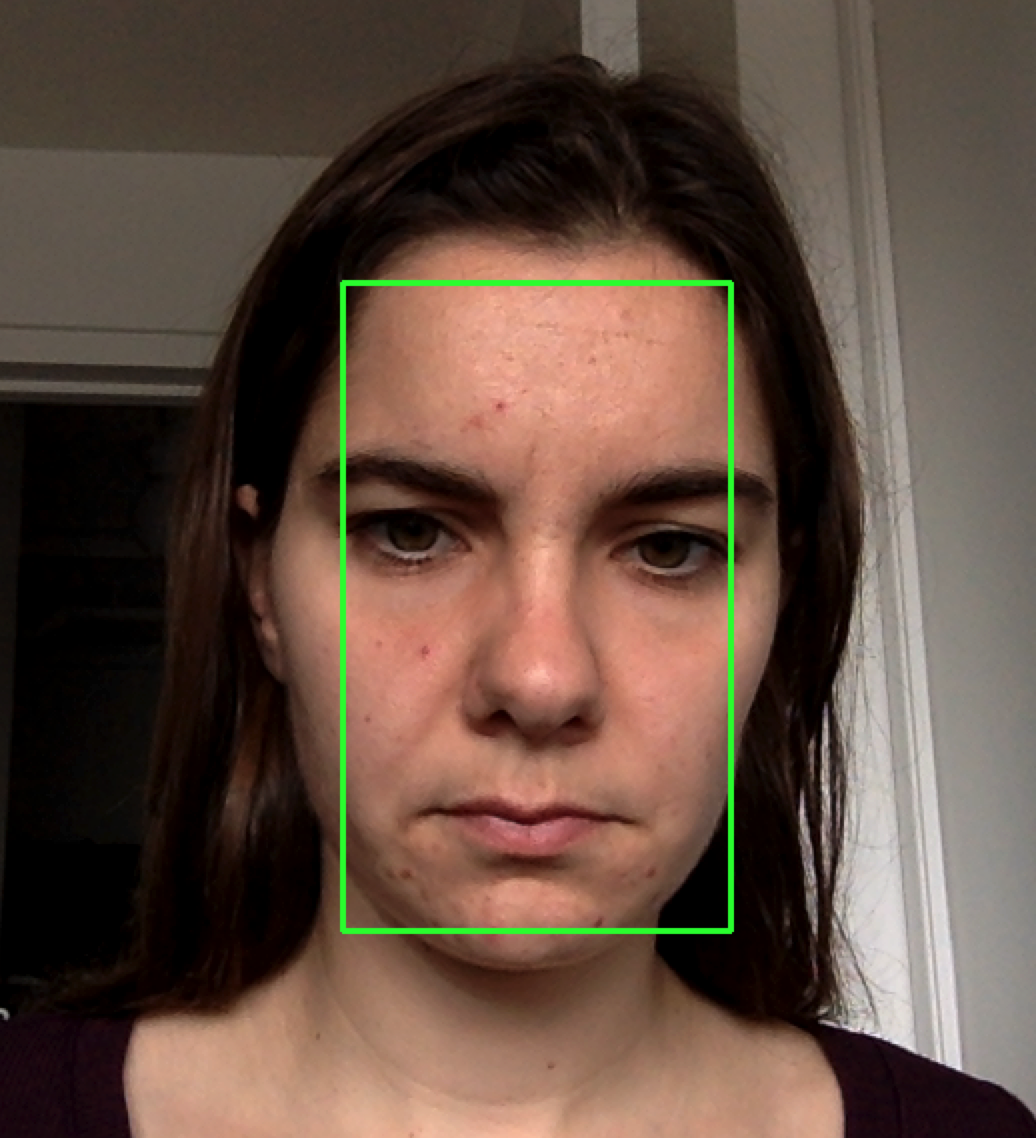
\includegraphics[scale=0.2]{face_bb}
\end{center}
\caption{Bounding box around pixels used for heart rate detection (ROI).}
\label{face_bb}
\end{figure}

I implemented face detection and tracking in Python using the OpenCV Cascade Classifier pre-trained on frontal face images. I chose the best bounding box from those returned by the classifier as described in the technical approach. I then extracted the center 60\% of the width and full height as my ROI. As shown in figure \ref{face_bb}, the ROI accurately tracks the face and contains mostly skin pixels although there is also sometimes hair appearing at the corners.

\subsection*{Heart Rate Detection}

\begin{figure}
\begin{center}
	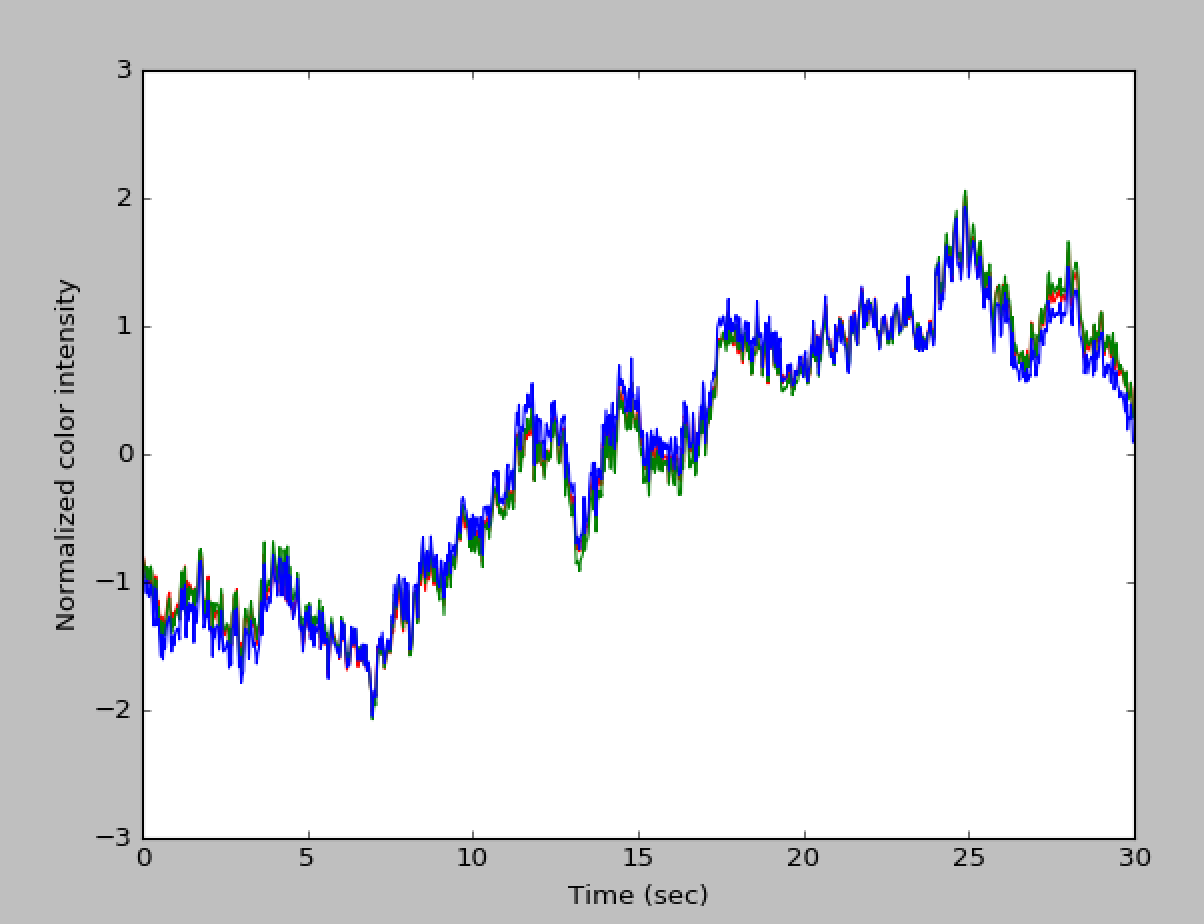
\includegraphics[scale=0.41]{rgb_signals}
	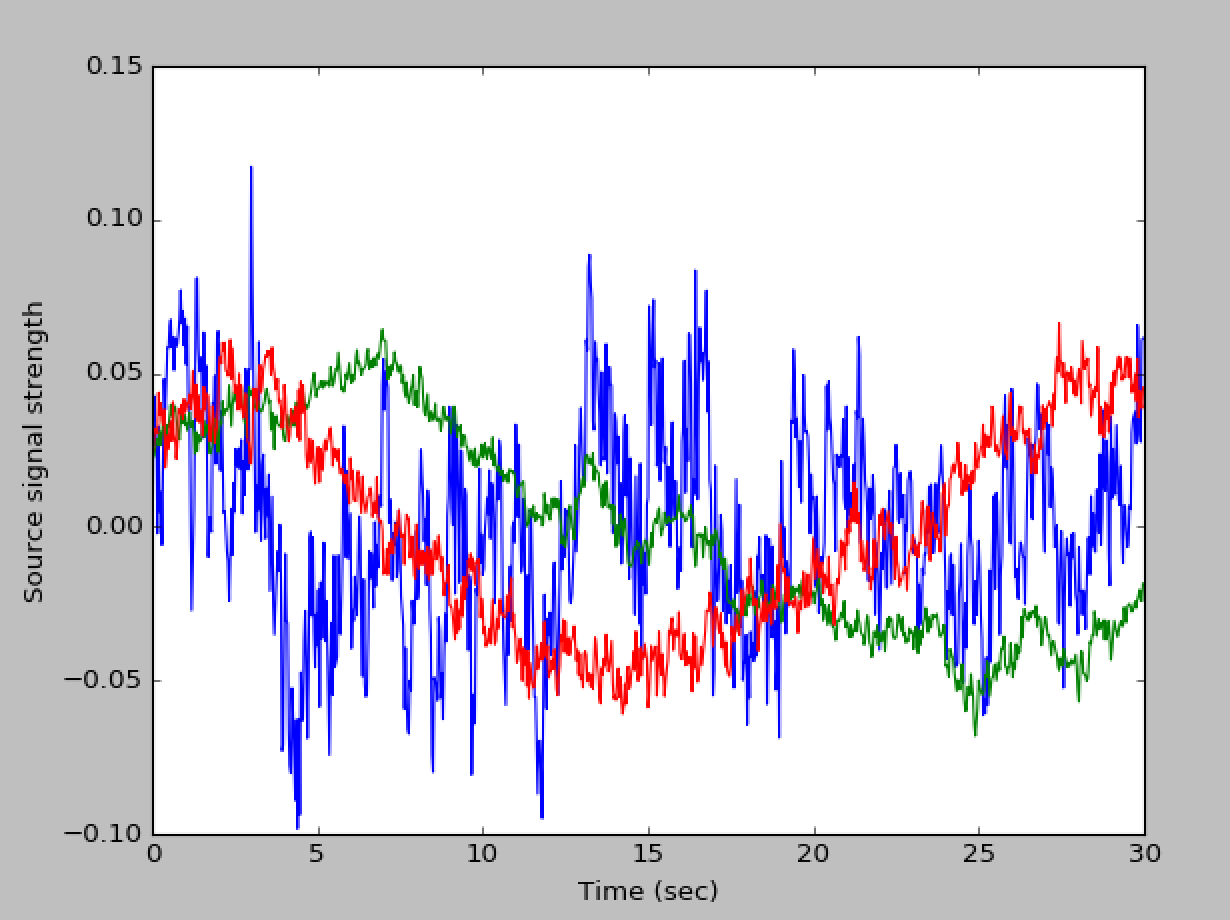
\includegraphics[scale=0.4]{src_signals}
\end{center}
\caption{Mean RGB color channel pixel values within the ROI (top) and associated source signals found through ICA (bottom) over a 30-second window.}
\label{time_plots}
\end{figure}

\begin{figure}
\begin{center}
	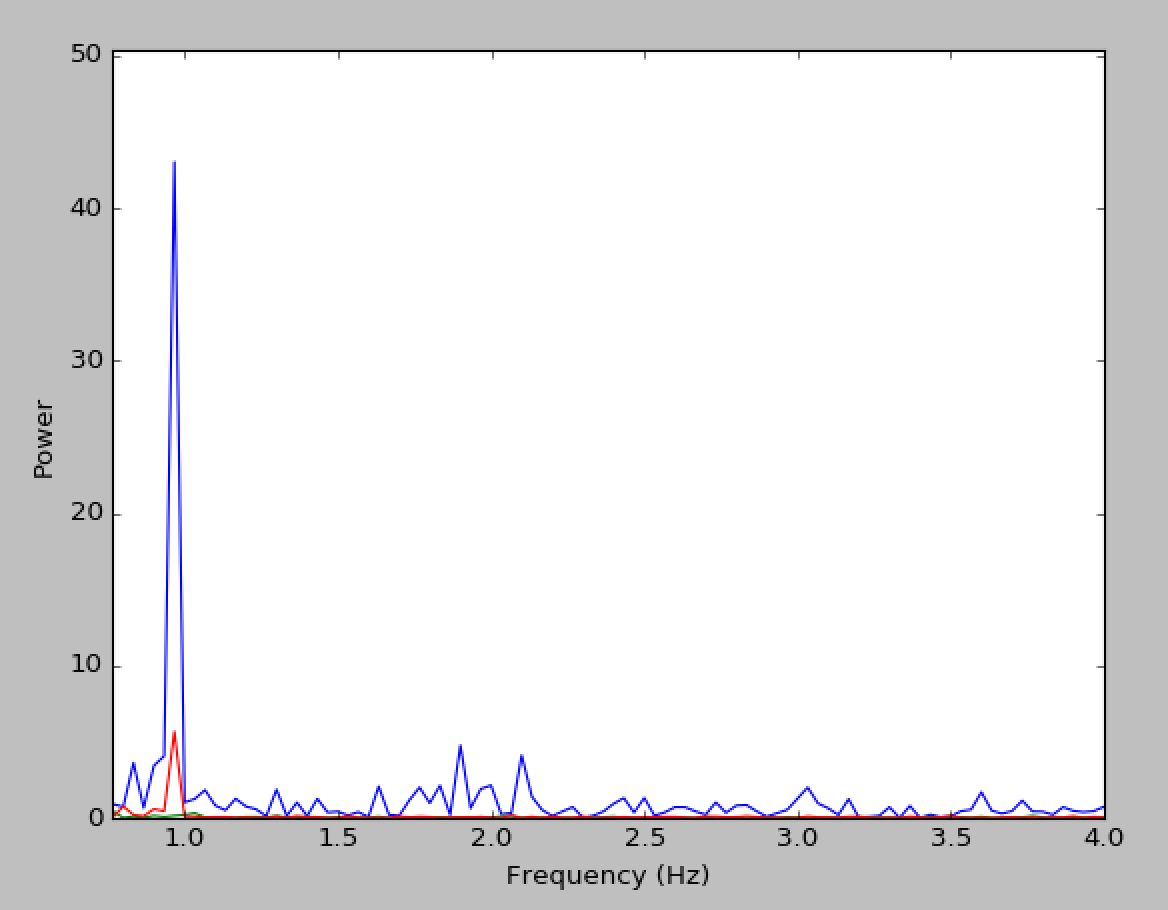
\includegraphics[scale=0.41]{pwr_spectrum}
\end{center}
\caption{Power spectrum for the three source signals over the physiological heart-rate range. The prominent frequency (0.97Hz) corresponds to a heart-rate of 58 bpm.}
\label{freq_plot}
\end{figure}

I extracted the heart rate signal from the ROI as described in the technical approach section. This process included pixel averaging across the ROI and then normalization across a sliding window, ICA to extract independent source signals, and power spectrum analysis to determine the prominent frequencies.

Figure \ref{time_plots} shows the normalized mean pixel intensity for the three color channels during a 30-second window as well as the three source signals found through ICA. Figure \ref{freq_plot} shows the power spectra for the three source signals within the physiological heart rate range. Although the strongest frequency in this range is just under 1 Hz, which corresponds to my approximate resting heart rate of 60 bpm, further experiments are required to ensure this is correctly picking up my heart rate and not some other signal or video artifact.

\section*{Remaining Milestones}

The first step going forward will be to ensure that I can accurately extract heart rate using videos of still faces. I will test my current implementation on a video of myself after exercising to see if the predicted heart rate increases. If I find that it is not tracking heart rate, I may try these videos in an implementation of the Eulerian small motion amplification software from Wu \etal~\cite{Wu:2012aa}. If the heart rate cannot be amplified, it may indicate an issue with the video format or frame rate.

Once I am confident I am measuring heart rate, I could more precisely test the accuracy of the measurements by comparing to a ground truth measurement. I have ordered a DIY photo-plethysmography sensor, which should arrive late this week. This PPG sensor uses an infrared photodiode and photodetector to measure changes in light transmission in the fingertip and outputs the raw pulse wave signal. I will connect the output to an analog-to-digital converter and then to a Raspberry Pi or Arduino to collect the digitized signal. I will then find the prominent frequency (heart rate) by analyzing the power spectrum, just as in the final step of the heart rate detection from video. I will then take videos of myself and others while wearing this PPG sensor so that I can compare results from the two methods.

The final step will be to test and potentially improve the heart rate results from video where the subject is not completely still. I will first test the accuracy on moving faces using the current implementation of face detection and ROI calculation. If the accuracy drops when movement is introduced, I will attempt to improve the accuracy through enhanced tracking and/or improved face segmentation, as described in the technical approach section.

Remaining milestone deadlines:

\begin{table}[h]
\centering
\begin{tabular}{ll}
	Ensure heart rate (HR) being detected 				& May 16\\
	Extract reference HR from PPG sensor and compare	& May 20\\
	Potential face tracking/segmentation improvements 		& May 27\\
	Project presentation 								& June 1\\
	Project paper 									& June 6\\
\end{tabular}
\end{table}

%-------------------------------------------------------------------------------
%\newpage

{\small
\bibliographystyle{ieee}
\bibliography{egbib}
}

\end{document}
